\documentclass[border=12pt]{standalone}
\usepackage{tikz}
\usetikzlibrary{shapes.geometric, arrows.meta, positioning, calc, fit, backgrounds}
\usepackage{fontspec}
\setmainfont{DejaVu Sans}

\begin{document}
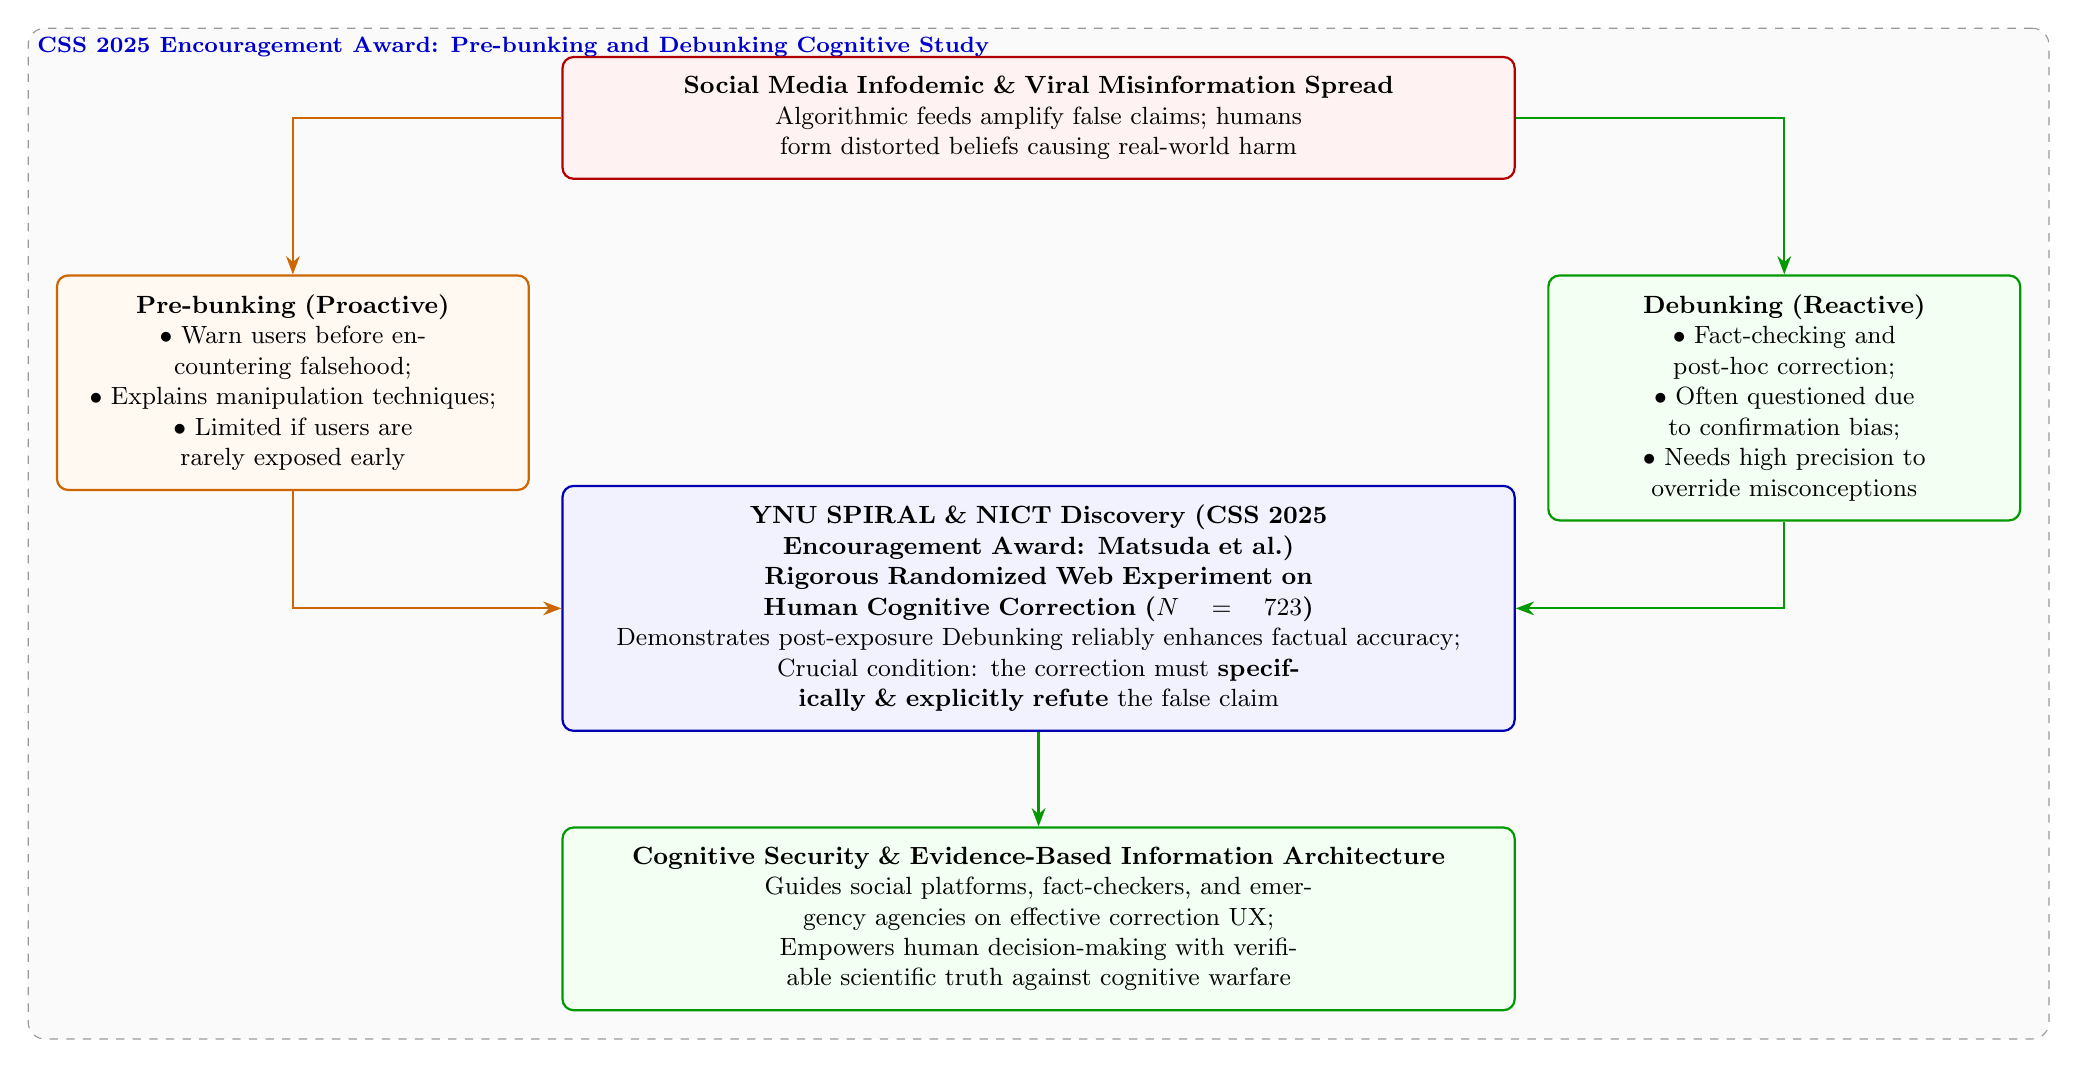
\begin{tikzpicture}[
    font=\small,
    >=Stealth,
    node distance=1.2cm,
    block/.style={rectangle, draw=blue!70!black, fill=blue!5, rounded corners=4pt, thick, align=center, inner sep=7pt},
    alertblock/.style={rectangle, draw=red!70!black, fill=red!5, rounded corners=4pt, thick, align=center, inner sep=7pt},
    greenblock/.style={rectangle, draw=green!60!black, fill=green!5, rounded corners=4pt, thick, align=center, inner sep=7pt},
    amberblock/.style={rectangle, draw=orange!80!black, fill=orange!5, rounded corners=4pt, thick, align=center, inner sep=7pt},
    groupbox/.style={draw=black!40, dashed, rounded corners=6pt, fill=black!2, inner sep=10pt}
]

    % Top: The Infodemic & Misinformation Crisis
    \node[alertblock, text width=11.6cm] (crisis) {\textbf{Social Media Infodemic \& Viral Misinformation Spread}\\Algorithmic feeds amplify false claims; humans form distorted beliefs causing real-world harm};

    % Left: Pre-bunking (Proactive Inoculation)
    \node[amberblock, below left=1.2cm and 0.4cm of crisis, text width=5.5cm] (prebunk) {\textbf{Pre-bunking (Proactive)}\\$\bullet$ Warn users before encountering falsehood;\\$\bullet$ Explains manipulation techniques;\\$\bullet$ Limited if users are rarely exposed early};

    % Right: Debunking (Reactive Correction)
    \node[greenblock, below right=1.2cm and 0.4cm of crisis, text width=5.5cm] (debunk) {\textbf{Debunking (Reactive)}\\$\bullet$ Fact-checking and post-hoc correction;\\$\bullet$ Often questioned due to confirmation bias;\\$\bullet$ Needs high precision to override misconceptions};

    \draw[->, thick, orange!80!black] (crisis) -| (prebunk);
    \draw[->, thick, green!60!black] (crisis) -| (debunk);

    % Middle: YNU & NICT Empirical Study (CSS 2025 Award)
    \node[block, below=1.2cm of $(prebunk)!0.5!(debunk)$, text width=11.6cm] (breakthrough) {\textbf{YNU SPIRAL \& NICT Discovery (CSS 2025 Encouragement Award: Matsuda et al.)}\\\textbf{Rigorous Randomized Web Experiment on Human Cognitive Correction ($N=723$)}\\Demonstrates post-exposure Debunking reliably enhances factual accuracy;\\Crucial condition: the correction must \textbf{specifically \& explicitly refute} the false claim};

    \draw[->, thick, orange!80!black] (prebunk) |- (breakthrough);
    \draw[->, thick, green!60!black] (debunk) |- (breakthrough);

    % Bottom: Societal Impact
    \node[greenblock, below=1.2cm of breakthrough, text width=11.6cm] (impact) {\textbf{Cognitive Security \& Evidence-Based Information Architecture}\\Guides social platforms, fact-checkers, and emergency agencies on effective correction UX;\\Empowers human decision-making with verifiable scientific truth against cognitive warfare};

    \draw[->, thick, green!60!black] (breakthrough) -- (impact);

    \begin{scope}[on background layer]
        \node[groupbox, fit=(crisis) (prebunk) (debunk) (breakthrough) (impact), label={[anchor=north west, font=\footnotesize\bfseries, blue!80!black]north west:CSS 2025 Encouragement Award: Pre-bunking and Debunking Cognitive Study}] {};
    \end{scope}

\end{tikzpicture}
\end{document}
